\documentclass[12pt]{article}
\usepackage{amsmath}
\usepackage{graphicx}
\usepackage{hyperref}
\usepackage[latin1]{inputenc}

\usepackage{verbatim}


\title{Lab 1 Report}
\author{Sam Spice}
\date{29/9/2018}

\begin{document}
\maketitle

\section{Intro}

This report contains an analysis of basic transmission rate analysis on a variety of networks with various configurations. Additionally this report contains basic analysis of queuing theory and a comparison between empirical data and theoretical models of queuing theory.

\section{Two Nodes}
The first set of experiments was conducted to test the transmission of packets across a 2 node network with a single connection. Various network configurations were adjusted, namely tranmission speed and propagation distance. The transmission speeds varied from 1Mbps to 100bps. Propagation Delays varied from 1 second to 10 miliseconds.

\subsection{Network Configurations}

Below are the contents of the network configuration files.
\linebreak
\centerline{fast-long.txt}
\verbatiminput{../../lab1a/networks/fast-long.txt}

\centerline{slow-short.txt}
\verbatiminput{../../lab1a/networks/slow-short.txt}

\centerline{fast-short.txt}
\verbatiminput{../../lab1a/networks/fast-short.txt}

\subsection{Simulation Output}
\begin{verbatim}
***Scenario 1***
(1, 0, 1.008)
***Scenario 2***
(1, 0, 80.01)
***Scenario 3***
(1, 0, 0.018000000000000002)
(2, 0, 0.026000000000000002)
(3, 0, 0.034)
(4, 2.0, 2.018)
\end{verbatim}

\subsection{Calculations}

The following section details the calculations used to verify that the output of the simulations, seen above, is correct. 

\centerline{Scenario 1 Calculation}
In the first scenario 2 nodes are connected by a fast link, transmitting at 1Mpbs, over a far distance, 1 second worth of propagation time. A single packet was sent across this network.
\begin{equation}
arrival time = D_{prop} + D_{transmission}
\end{equation}
\centerline{Transmission Delay}
\begin{equation}
D_{transmission} = 8000 / (10^6) = .008
\end{equation}
\begin{equation}
1.008 = 1_{second} + .008_{seconds}
\end{equation}


\centerline{Scenario 2 Calculation}
In the second scenario 2 nodes are connected by a slow link, 100bps, over a short distance, 10ms worth of propagation time. A single packet was sent across this network.
\begin{equation}
arrival time = D_{prop} + D_{transmission}
\end{equation}
\centerline{Transmission Delay}
\begin{equation}
D_{transmission} = 8000 / (100) = .80
\end{equation}
\begin{equation}
.018 = .01_{seconds} + .80_{seconds}
\end{equation}

\centerline{Scenario 3 Calculations}
In the third scenario 2 nodes are connected by a fast link, 1Mbps, over a short distance, 10ms worth of propation time. 4 packets were sent across this network, 3 in quick succession then a final packet sent 2 seconds after the simulation began.
\begin{equation}
arrival time = D_{prop} + (D_{transmission} * Packet Number)
\end{equation}
\centerline{Transmission Delay}
\begin{equation}
D_{transmission} = 8000 / (10^6) = .008
\end{equation}

\centerline{First Packet Arrival time}
\begin{equation}
 .018 = .01_{second} + .008_{seconds}
\end{equation}

\centerline{Second Packet Arrival time}
\begin{equation}
  0.024 = .01_{second} + (.008_{seconds} * 2)
\end{equation}

\centerline{Third Packet Arrival time}
\begin{equation}
  0.034 = .01_{second} + (.008_{seconds} * 3)
\end{equation}

\centerline{Fourth Packet Arrival time}
\begin{equation}
arrival_time = D_{prop} + D_{transmission} + Delay
\end{equation}
\begin{equation}
  2.018 = .01_{second} + .008_{seconds} + 2
\end{equation}

\subsection{Two Node Wrapup}
As seen in the experiments above two node network calculations are very straightforward and the experiments did not yield any unexpected or surprising results. The experiment did prove that experimental results matched theoretical results perfectly.



\section{Three Nodes}
In the second set of experiments conducted 10000 packets were sent across a 3 node network consisting of 2 spans connecting the 3 nodes. These packets were all 1000 bytes in size and sent back to back as quickly as possible. 

\subsection{Network Configurations}
Below are the contents of the various network configuration files.\\

\centerline{fast-fast.txt}
\verbatiminput{../../lab1a/networks/fast-fast.txt}

\centerline{faster-faster.txt}
\verbatiminput{../../lab1a/networks/faster-faster.txt}

\centerline{faster-slow.txt}
\verbatiminput{../../lab1a/networks/fast-slow.txt}

\subsection{Simulation Output}
Below is the output of the simulation. The results here appear exactly as they appear in the console following execution of the simulations.\\
\centerline{Simulation 1 Output}
\begin{verbatim}
(9996, 79.96000000000001, 80.17600000000185, 0.21600000000184139, 0.016, 0.2, 1.8332002582610585e-12)
(9997, 79.968, 80.18400000000184, 0.21600000000184139, 0.016, 0.2, 1.8332002582610585e-12)
(9998, 79.976, 80.19200000000184, 0.21600000000184139, 0.016, 0.2, 1.8332002582610585e-12)
(9999, 79.984, 80.20000000000184, 0.21600000000184139, 0.016, 0.2, 1.8332002582610585e-12)
(10000, 79.992, 80.20800000000183, 0.21600000000182717, 0.016, 0.2, 1.8189894035458565e-12)
\end{verbatim}

\centerline{Simulation 2 Output}
\begin{verbatim}
(9996, 0.07996, 0.27997600000005624, 0.20001600000005623, 1.6e-05, 0.2, 5.620504062164855e-14)
(9997, 0.079968, 0.27998400000005624, 0.20001600000005626, 1.6e-05, 0.2, 5.623279619726418e-14)
(9998, 0.07997599999999999, 0.27999200000005625, 0.20001600000005626, 1.6e-05, 0.2, 5.626055177287981e-14)
(9999, 0.079984, 0.28000000000005626, 0.20001600000005626, 1.6e-05, 0.2, 5.626055177287981e-14)
(10000, 0.079992, 0.28000800000005627, 0.20001600000005626, 1.6e-05, 0.2, 5.626055177287981e-14)
\end{verbatim}

\centerline{Simulation 3 Output}
\begin{verbatim}
(9996, 79.96000000000001, 312.583, 232.62300000000002, 0.03925, 0.2, 232.38374999999996)
(9997, 79.968, 312.61425, 232.64625, 0.03925, 0.2, 232.40699999999998)
(9998, 79.976, 312.6455, 232.66950000000003, 0.03925, 0.2, 232.43025)
(9999, 79.984, 312.67675, 232.69275000000005, 0.03925, 0.2, 232.45350000000002)
(10000, 79.992, 312.708, 232.716, 0.03925, 0.2, 232.47674999999998)
\end{verbatim}

\subsection{Calculations}
Below are the calculations used to verify that the results of simulation 3 are correct\\
\centerline{Simulation 1 Calculations}

\begin{equation}
D_{transmission} = 8000 / (10^6) = .008
\end{equation}
\begin{equation}
\begin{split}
SinglePacketTransmission = ( D_{transmission} * 2) + (D_{prop} * 2) \\= (.008 * 2) + (.1 * 2) = .216
\end{split}
\end{equation}
\begin{equation}
\begin{split}
TotalTransmissionTime = (10001 * D_{transmission}) + (2 * D_{prop}) \\= 80.208 seconds
\end{split}
\end{equation}

\centerline{Simulation 2 Calculations}

\begin{equation}
D_{transmission} = 8000 / (10^9) = .000008
\end{equation}
\begin{equation}
\begin{split}
SinglePacketTransmission = ( D_{transmission} * 2) + (D_{prop} * 2) \\= (.000008 * 2) + (.1 * 2) = .200016
\end{split}
\end{equation}
\begin{equation}
\begin{split}
TotalTransmissionTime = (10001 * D_{transmission}) + (2 * D_{prop}) \\= .280008 seconds
\end{split}
\end{equation}

\centerline{Simulation 3 Calculations}
\begin{equation}
D_{transmission-second-link} = 8000 / (256000) = .03125
\end{equation}
\begin{equation}
D_{transmission-first-link} = 8000 / (10^9) = .000008
\end{equation}
\begin{equation}
\begin{split}
SinglePacketTransmission =\\ ( D_{transmission-first-link} + D_{transmission-second-link}  + (D_{transmission} * 2) \\= .000008 + .03125 + (.1 * 2) = .231258
\end{split}
\end{equation}
\begin{equation}
\begin{split}
TotalTransmissionTime =\\ (1000 * D_{transmission-second-link}) + D_{transmission-first-link} + (2 * D_{prop}) \\= 312.708 seconds
\end{split}
\end{equation}

\subsection{Three Node Wrapup}
As seen in the output of the experiments we see that the transmission delay dominates the overall transmission time for 10,000 packets on a network with relatively fast propagation speed. The third simulation shows this clearly as the overally time was dominated entirely by the slower transmission time. The first link could have been near instantaneous and it would would not have increased the overall time to transmit 10,000 packets. As the number of packets increases transmission delay grows more important and propagation delay become less important. 

\section{Delay Experiments}
In the third and final experiment rudimentary queuing theory was tested to see how accuratly empirical data gathered about average queue delays matched theoretical expectations\\
Graphs were generated to compare these two sets of results, these graphs can be seen below\\

\subsection{Network Configuration}
\centerline{fast-fast.txt}
\verbatiminput{../../lab1a/networks/fast-fast.txt}

\subsection{Packet Generation loads}
In order to accurately generate packets to be sent across the network with a given distribution based on the given Lambda.\\
Lambdas were generated for a given p by the following formula\\
\begin{equation}
mu = 1000000 // (1000 * 8)
\end{equation}
\begin{equation}
lambda = p * mu
\end{equation} 

\subsection{Graph}
As seen in the graph below the theoretical and empirical plots are almost entirely overlapping showing that basic queuing theory principles hold up when looked at under scrutiny. This graph shows the value of basic queuing theory equations and negates the need for large scale experiments when the theoretical numbers are so incredibly close to the experimental.\\
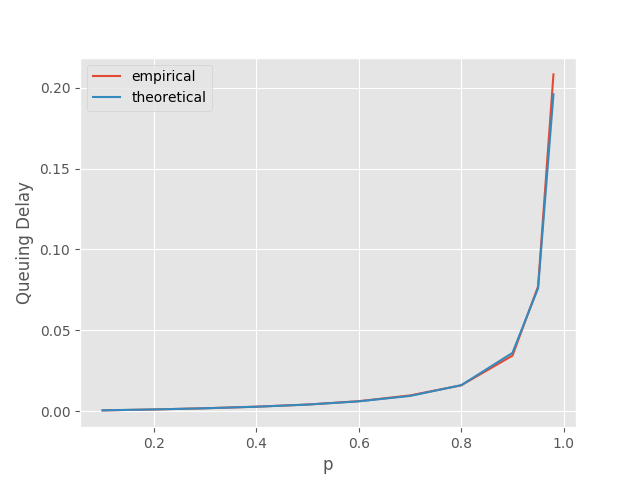
\includegraphics[scale=.75]{../graphs/delay.png}

\section{Conlusion}
The experiments conducted provided valuable insight into simple network analysis as well as data gathered from more complex networks with many more packets being sent across the networks. Additionally the experiments provided valuable insight into the basics of queuing theory and illustrated that as link utilization approaches 1 the average queuing delay for packets increases towards infinity, illustrating that if a link is overly crowded then packets will start getting dropped and message will be lost entirely. 


\end{document}

